\documentclass[11pt]{report}

\usepackage{amsmath}
\usepackage{hyperref}
\usepackage{graphicx}
\usepackage{listings}
\usepackage{color}

\author{
  OJAS APOORVA KANHERE\\
  \texttt{12D070002}
  \and
  PRAVEEN AGRAWAL\\
  \texttt{12D020030}
  \and
  KOTWAL ALANKAR SHASHIKANT\\
  \texttt{12D070010}
}
\title{EE 337 / EE 309 - Microprocessor Design Report}

\definecolor{mygreen}{rgb}{0,0.6,0}
\definecolor{mygray}{rgb}{0.5,0.5,0.5}
\definecolor{mymauve}{rgb}{0.58,0,0.82}

\lstset{ %
  backgroundcolor=\color{white},   % choose the background color; you must add \usepackage{color} or \usepackage{xcolor}
  basicstyle=\footnotesize,        % the size of the fonts that are used for the code
  breakatwhitespace=false,         % sets if automatic breaks should only happen at whitespace
  breaklines=true,                 % sets automatic line breaking
  captionpos=b,                    % sets the caption-position to bottom
  commentstyle=\color{mygreen},    % comment style
  deletekeywords={...},            % if you want to delete keywords from the given language
  escapeinside={\%*}{*)},          % if you want to add LaTeX within your code
  extendedchars=true,              % lets you use non-ASCII characters; for 8-bits encodings only, does not work with UTF-8
  frame=single,                    % adds a frame around the code
  keepspaces=true,                 % keeps spaces in text, useful for keeping indentation of code (possibly needs columns=flexible)
  keywordstyle=\color{blue},       % keyword style
  language=Verilog,                 % the language of the code
  morekeywords={*,...},            % if you want to add more keywords to the set
  numbers=left,                    % where to put the line-numbers; possible values are (none, left, right)
  numbersep=5pt,                   % how far the line-numbers are from the code
  numberstyle=\tiny\color{mygray}, % the style that is used for the line-numbers
  rulecolor=\color{black},         % if not set, the frame-color may be changed on line-breaks within not-black text (e.g. comments (green here))
  showspaces=false,                % show spaces everywhere adding particular underscores; it overrides 'showstringspaces'
  showstringspaces=false,          % underline spaces within strings only
  showtabs=false,                  % show tabs within strings adding particular underscores
  stepnumber=2,                    % the step between two line-numbers. If it's 1, each line will be numbered
  stringstyle=\color{mymauve},     % string literal style
  tabsize=2,                       % sets default tabsize to 2 spaces
  title=\lstname                   % show the filename of files included with \lstinputlisting; also try caption instead of title
}

\begin{document}

\maketitle

\section*{1 Introduction}
The aim of this exercise was to design and implement an 8-bit RISC processor on an FPGA. The ISA used was the LC-3b instruction set. You may find the instruction set \href{http://users.ece.utexas.edu/~patt/11s.460N/handouts/new_byte.pdf}{here}.

In RISC design, we have to choose between a multi-cycle implementation and a single-cycle implementation. We chose to implement a multi-cycle data-path because all instructions do not take an equal amount of time, and the multi-cycle implementation makes sure that each instruction gets over in the minimum amount of time it requires. Also the single-cycle data-path is more complicated as compared to the multi-cycle data-path, and we save significant resources on the FPGA by doing a multi-cycle implementation.

You may find all the code for our project \href{http://www.github.com/AlankarKotwal/lc-3b-processor}{here}

\section*{2 Data-path}
The data-path we designed is summarised in the diagram below.\newline
\newline
\centerline{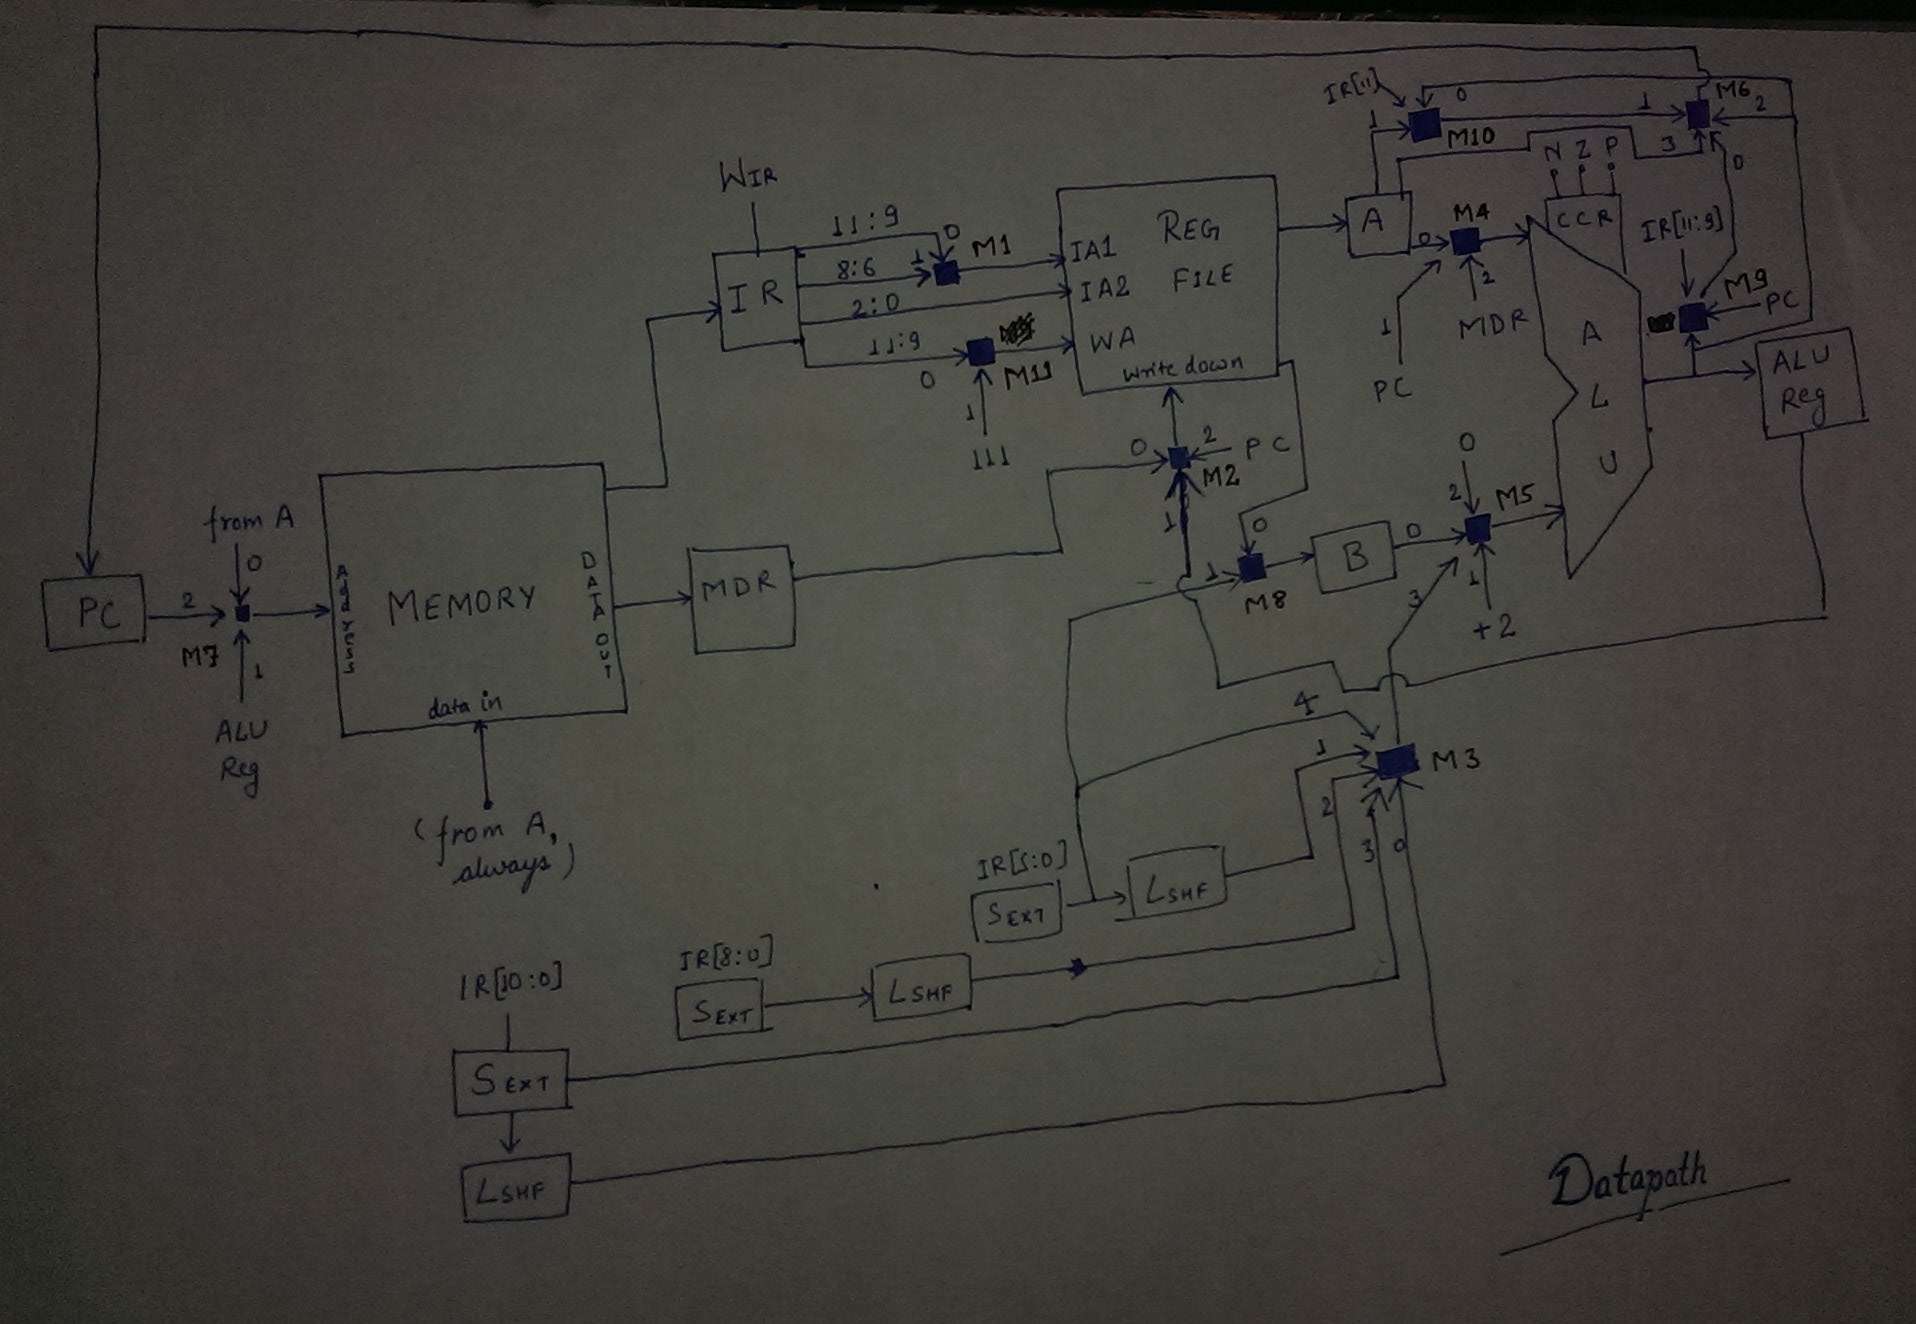
\includegraphics[scale=0.20]{datapath.jpg}}
\newline

\section*{3 Controller}
The controller implemented has two parts: logic driving current control signals and next state logic. The code for the current control signal values is as follows:

\begin{lstlisting}
always@(*) begin
	case(StateID)
		1: begin
			Mux1 = 1'b1;
			Mux2 = 2'b11;
			Mux3 = 3'b111;
			Mux4 = 2'b01;
			Mux5 = 2'b01;
			Mux6 = 2'b10;
			Mux7 = 2'b10;
			Mux11 = 1'b1;

			wrf = 1'b1;
			wpc = ~|IR;
			wir = 1'b0;
			lccr = 1'b1;
			aluop = 2'b00;
			alushop = 2'b11;
			wmem = 1'b1;
			wa = 1'b1;
			wb = 1'b1;
			lalu = 1'b1;
		end
			
		2: begin
			Mux1 = 1'b1;
			Mux2 = 2'b11;
			Mux3 = 3'b111;
			Mux4 = 2'b11;
			Mux5 = 2'b11;
			Mux6 = 2'b11;
			Mux7 = 2'b11;
			Mux11 = 1'b1;

			wrf = 1'b1;
			wpc = 1'b1;
			wir = 1'b1;
			lccr = 1'b1;
			aluop = 2'b11;
			alushop = 2'b11;
			wmem = 1'b1;
			wa = 1'b0;
			wb = 1'b0;
			lalu = 1'b1;
		end
			
		3: begin
			Mux1 = 1'b1;
			Mux2 = 2'b11;
			Mux3 = 3'b111;
			Mux4 = 2'b00;
			Mux5 = 2'b00;
			Mux6 = 2'b11;
			Mux7 = 2'b11;
			Mux11 = 1'b1;
			 
			wrf = 1'b1;
			wpc = 1'b1;
			wir = 1'b1;
			lccr = 1'b0;
			aluop = {IR[15], IR[14]};
			alushop = {IR[5], IR[4]};
			wmem = 1'b1;
			wa = 1'b1;
			wb = 1'b1;
			lalu = 1'b0;
		end
			
		4: begin
			Mux1 = 1'b1;
			Mux2 = 2'b01;
			Mux3 = 3'b111;
			Mux4 = 2'b11;
			Mux5 = 2'b11;
			Mux6 = 2'b11;
			Mux7 = 2'b11;
			Mux11 = 1'b0;
			 
			wrf = 1'b0;
			wpc = 1'b1;
			wir = 1'b1;
			lccr = 1'b1;
			aluop = 2'b11;
			alushop = 2'b11;
			wmem = 1'b1;
			wa = 1'b1;
			wb = 1'b1;
			lalu = 1'b1;
		end
		
		5: begin
			Mux1 = 1'b1;
			Mux2 = 2'b11;
			Mux3 = 3'b010;
			Mux4 = 2'b01;
			Mux5 = 2'b11;
			Mux6 = 2'b00;
			Mux7 = 2'b11;
			Mux11 = 1'b1;
			 
			wrf = 1'b1;
			wpc = 1'b0;
			wir = 1'b1;
			lccr = 1'b1;
			aluop = 2'b00;
			alushop = 2'b11;
			wmem = 1'b1;
			wa = 1'b1;
			wb = 1'b1;
			lalu = 1'b1;
		end
			
		6: begin
			Mux1 = 1'b1;
			Mux2 = 2'b11;
			Mux3 = 3'b111;
			Mux4 = 2'b11;
			Mux5 = 2'b11;
			Mux6 = 2'b11;
			Mux7 = 2'b11;
			Mux11 = 1'b1;
			 
			wrf = 1'b1;
			wpc = 1'b0;
			wir = 1'b1;
			lccr = 1'b1;
			aluop = 2'b11;
			alushop = 2'b11;
			wmem = 1'b1;
			wa = 1'b1;
			wb = 1'b1;
			lalu = 1'b1;
		end
			
		7: begin
			Mux1 = 1'b1;
			Mux2 = 2'b10;
			Mux3 = 3'b111;
			Mux4 = 2'b11;
			Mux5 = 2'b11;
			Mux6 = 2'b11;
			Mux7 = 2'b11;
			Mux11 = 1'b1;
			 
			wrf = 1'b0;
			wpc = 1'b1;
			wir = 1'b1;
			lccr = 1'b1;
			aluop = 2'b11;
			alushop = 2'b11;
			wmem = 1'b1;
			wa = 1'b1;
			wb = 1'b1;
			lalu = 1'b1;
		end
			
		8: begin
			Mux1 = 1'b1;
			Mux2 = 2'b11;
			Mux3 = 3'b000;
			Mux4 = 2'b01;
			Mux5 = 2'b11;
			Mux6 = 2'b01;
			Mux7 = 2'b11;
			Mux11 = 1'b1;
			 
			wrf = 1'b1;
			wpc = 1'b0;
			wir = 1'b1;
			lccr = 1'b1;
			aluop = 2'b00;
			alushop = 2'b11;
			wmem = 1'b1;
			wa = 1'b1;
			wb = 1'b1;
			lalu = 1'b1;
		end
			
		9: begin
			Mux1 = 1'b1;
			Mux2 = 2'b11;
			Mux3 = 3'b100;
			Mux4 = 2'b00;
			Mux5 = 2'b11;
			Mux6 = 2'b11;
			Mux7 = 2'b11;
			Mux11 = 1'b1;
			 
			wrf = 1'b1;
			wpc = 1'b1;
			wir = 1'b1;
			lccr = 1'b1;
			aluop = 2'b00;
			alushop = 2'b11;
			wmem = 1'b1;
			wa = 1'b1;
			wb = 1'b1;
			lalu = 1'b0;
		end
			
		10: begin
			Mux1 = 1'b0;
			Mux2 = 2'b11;
			Mux3 = 3'b111;
			Mux4 = 2'b11;
			Mux5 = 2'b11;
			Mux6 = 2'b11;
			Mux7 = 2'b11;
			Mux11 = 1'b1;

			wrf = 1'b1;
			wpc = 1'b1;
			wir = 1'b1;
			lccr = 1'b1;
			aluop = 2'b11;
			alushop = 2'b11;
			wmem = 1'b1;
			wa = 1'b0;
			wb = 1'b1;
			lalu = 1'b1;
		end
			
		11: begin
			Mux1 = 1'b1;
			Mux2 = 2'b11;
			Mux3 = 3'b111;
			Mux4 = 2'b11;
			Mux5 = 2'b11;
			Mux6 = 2'b11;
			Mux7 = 2'b01;	
			Mux11 = 1'b1;
			 
			wrf = 1'b1;
			wpc = 1'b1;
			wir = 1'b1;
			lccr = 1'b1;
			aluop = 2'b11;
			alushop = 2'b11;
			wmem = 1'b0;
			wa = 1'b1;
			wb = 1'b1;
			lalu = 1'b1;
		end
		
		12:begin
			Mux1 = 1'b1;
			Mux2 = 2'b11;
			Mux3 = 3'b001;
			Mux4 = 2'b00;
			Mux5 = 2'b11;
			Mux6 = 2'b11;
			Mux7 = 2'b11;
			Mux11 = 1'b1;
			 
			wrf = 1'b1;
			wpc = 1'b1;
			wir = 1'b1;
			lccr = 1'b1;
			aluop = 2'b00;
			alushop = 2'b11;
			wmem = 1'b1;
			wa = 1'b1;
			wb = 1'b1;
			lalu = 1'b0;
		end

		13:begin
			Mux1 = 1'b1;
			Mux2 = 2'b11;
			Mux3 = 3'b111;
			Mux4 = 2'b11;
			Mux5 = 2'b11;
			Mux6 = 2'b11;
			Mux7 = 2'b01;
			Mux11 = 1'b1;
			 
			wrf = 1'b1;
			wpc = 1'b1;
			wir = 1'b1;
			lccr = 1'b1;
			aluop = 2'b11;
			alushop = 2'b11;
			wmem = 1'b1;
			wa = 1'b1;
			wb = 1'b1;
			lalu = 1'b1;
		end
			
		14:begin
			Mux1 = 1'b1;
			Mux2 = 2'b00;
			Mux3 = 3'b111;
			Mux4 = 2'b10;
			Mux5 = 2'b10;
			Mux6 = 2'b11;
			Mux7 = 2'b01;
			Mux11 = 1'b0;
			 
			wrf = 1'b0;
			wpc = 1'b1;
			wir = 1'b1;
			lccr = 1'b0;
			aluop = 2'b00;
			alushop = 2'b11;
			wmem = 1'b1;
			wa = 1'b1;
			wb = 1'b1;
			lalu = 1'b1;
		end
			
		15:begin
			Mux1 = 1'b1;
			Mux2 = 2'b11;
			Mux3 = 3'b010;
			Mux4 = 2'b01;
			Mux5 = 2'b11;
			Mux6 = 2'b11;
			Mux7 = 2'b11;
			Mux11 = 1'b1;
			 
			wrf = 1'b1;
			wpc = 1'b1;
			wir = 1'b1;
			lccr = 1'b0;
			aluop = 2'b00;
			alushop = 2'b11;
			wmem = 1'b1;
			wa = 1'b1;
			wb = 1'b1;
			lalu = 1'b0;
		end
			
		16:begin
			Mux1 = 1'b1;
			Mux2 = 2'b01;
			Mux3 = 3'b111;
			Mux4 = 2'b11;
			Mux5 = 2'b11;
			Mux6 = 2'b11;
			Mux7 = 2'b11;
			Mux11 = 1'b0;
			 
			wrf = 1'b0;
			wpc = 1'b1;
			wir = 1'b1;
			lccr = 1'b1;
			aluop = 2'b11;
			alushop = 2'b11;
			wmem = 1'b1;
			wa = 1'b1;
			wb = 1'b1;
			lalu = 1'b1;
		end

		default: begin
			Mux1 = 1'b0;
			Mux2 = 2'b00;
			Mux3 = 3'b000;
			Mux4 = 2'b00;
			Mux5 = 2'b00;
			Mux6 = 2'b00;
			Mux7 = 2'b00;
			Mux11 = 1'b0;
			 
			wrf = 1'b1;
			wpc = 1'b1;
			wir = 1'b1;
			lccr = 1'b1;
			aluop = 2'b00;
			alushop = 2'b00;
			wmem = 1'b1;
			wa = 1'b1;
			wb = 1'b1;
			lalu = 1'b1;
		end
	endcase
end
\end{lstlisting}

where, the control signals mean the following:

\begin{center}
    \begin{tabular}{ | l | l | l | p{5cm} |}
    \hline
    No & Signal Name & Purpose \\ \hline
    1 & Mux1 & Mux1 Control Signal \\ \hline
    2 & Mux2 & Mux2 Control Signal \\ \hline
    3 & Mux3 & Mux3 Control Signal \\ \hline
    4 & Mux4 & Mux4 Control Signal \\ \hline
    5 & Mux5 & Mux5 Control Signal \\ \hline
    6 & Mux6 & Mux6 Control Signal \\ \hline
    7 & Mux7 & Mux7 Control Signal \\ \hline
    8 & Mux11 & Mux11 Control Signal \\ \hline
    9 & wrf & Write to Register File \\ \hline
    10 & wpc & Write to Program Counter \\ \hline
    11 & wir & Write to Instruction Register \\ \hline
    12 & lccr & Write to Condition Code Register \\ \hline
    13 & aluop & ALU Operation \\ \hline
    14 & alushop & Shift Operation \\ \hline
    15 & wmem & Write to Memory \\ \hline
    16 & wa & Write to Temporary Register A \\ \hline
    17 & wb & Write to Temporary Register B \\ \hline
    18 & lalu & Load ALU Register \\ \hline
    \end{tabular}
\end{center}

Mux8-Mux10 receive their inputs directly via combinational logic from IR. The logic is:
\begin{lstlisting}
Mux8  = IR[5];
Mux9  = ((IR[11]&&N)|| (IR[10]&&Z)||(IR[9]&&P));
Mux10 = IR[11];
\end{lstlisting}

\newpage
The next state logic is summarised in the following diagram:\newline \newline
\centerline{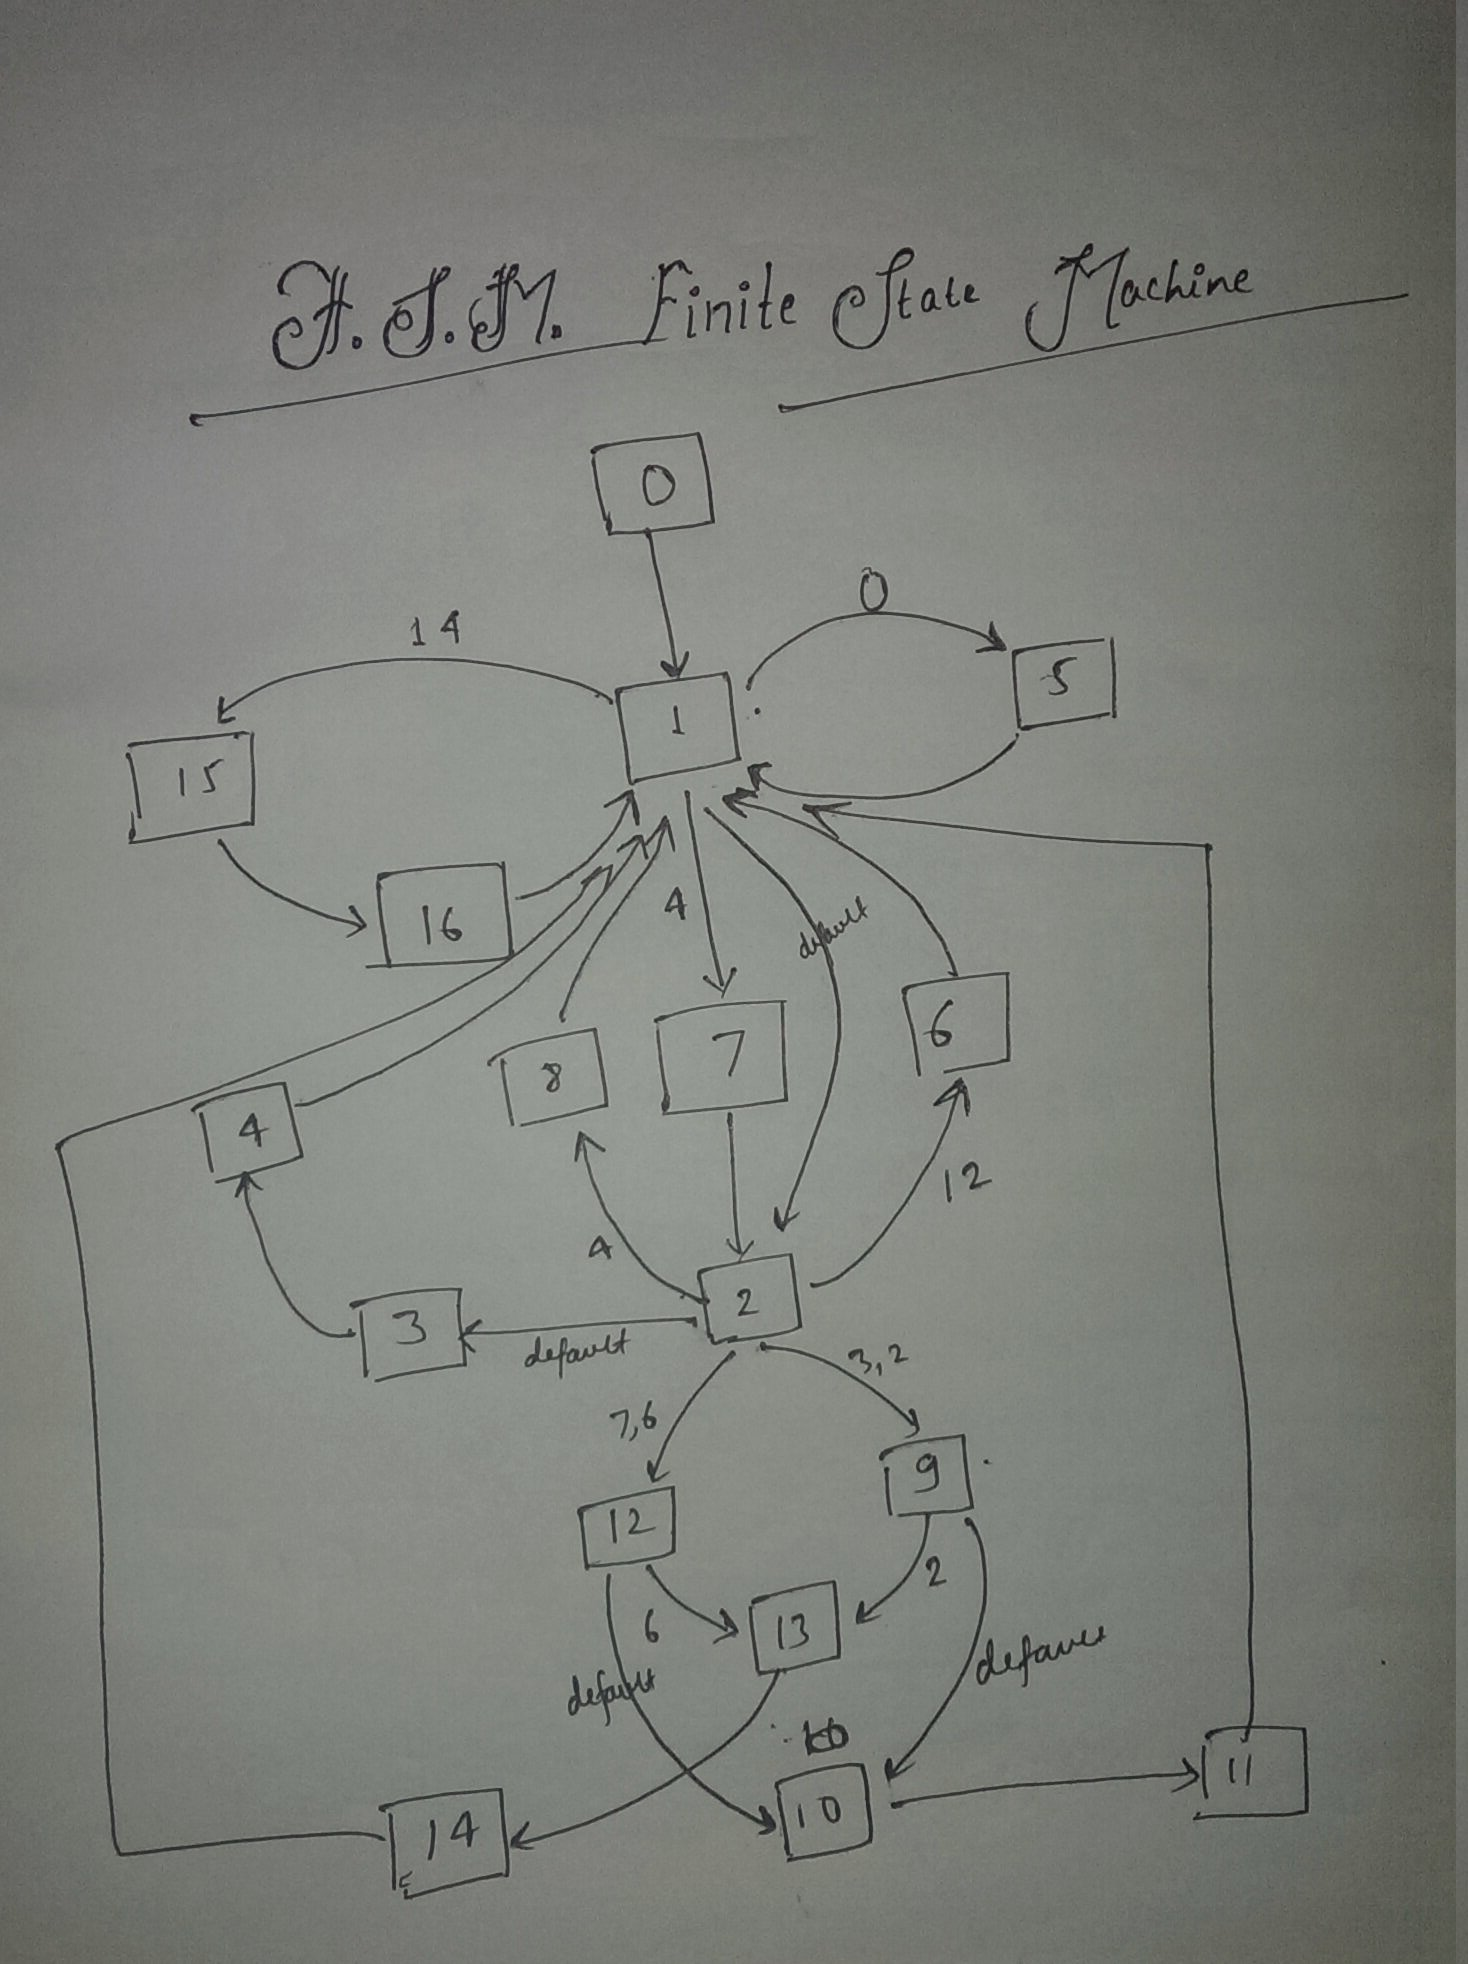
\includegraphics[scale=0.2]{controller.jpg}} \newline \newline
For each instruction the state sequence is shown below:
\newline
ALU Operation (Add, And, XOR, Not, Shifts): 1 $\rightarrow$ 2 $\rightarrow$ 3 $\rightarrow$ 4
\newline
Branch: 1 $\rightarrow$ 5
\newline
Call Subroutine: 1 $\rightarrow$ 7 $\rightarrow$ 2 $\rightarrow$ 8
\newline
Load Byte: 1 $\rightarrow$ 2 $\rightarrow$ 9 $\rightarrow$ 13 $\rightarrow$ 14
\newline
Load Word: 1 $\rightarrow$ 2 $\rightarrow$ 12 $\rightarrow$ 13 $\rightarrow$ 14
\newline
Load Immediate Address: 1 $\rightarrow$ 15 $\rightarrow$ 16
\newline
Store Byte: 1 $\rightarrow$ 2 $\rightarrow$ 9 $\rightarrow$ 10 $\rightarrow$ 11
\newline
Store Word: 1 $\rightarrow$ 2 $\rightarrow$ 12 $\rightarrow$ 10 $\rightarrow$ 11
\newline
\section*{4 Simulation}
We simulated the implementation using a test code that contained all the necessary functionality. In assembly language as per the LC-3b document, the code is as follows:

\begin{lstlisting}
NOT R1,R0
LDW R2,R0,#0
ADD R3,R2,R1
STW R3,R4,#7
LDB R7,R4,#14
BRp label

ORG 0x34
label:
JMP R7;
JSR label1

ORG 0x66
label1:
\end{lstlisting}

The simulation was carried out using GTKWave and iVerilog. The result for the above program were as shown below.
\newline
\centerline{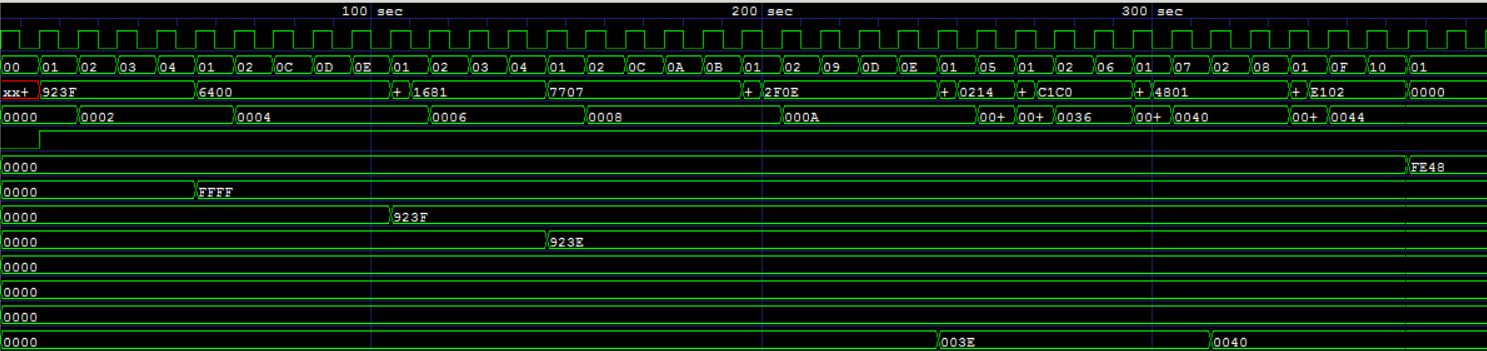
\includegraphics[scale=0.5]{gtkwave.png}}

\section*{5 Testing}
The implementation was tested on an Altera DE0-nano board having a Cyclone-IV FPGA. \newline
\centerline{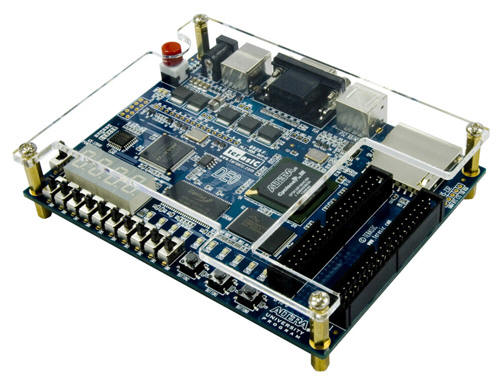
\includegraphics[scale=0.5]{de0.jpg}} \newline
The signal-tap tool was used to get states of the elements inside the FPGA at various points in time. For convenience in debugging we gave clock using a push-button on-board. The output was well as expected.

\end{document}